\section{The Induction Coupler System}
\label{sec:system}

The rotational speed of each array controls the force between that array and the surface of the target. The sum of the forces from all the arrays and their resultant torque can be mapped through the linearized dynamics of the target and chaser to plan control inputs based on a desired maneuver. Nonlinearities are likely best accommodated through gain scheduling, a topic that the authors intend to take up as future work.

With an operating range of a few centimeters, the surface for most of the ISS looks like an infinite plane to the inspection spacecraft. This analysis assumes that the proposed inspection vehicle conforms to the CubeSat standard so the mass of the entire system is not above m = 4 kg.
It is possible for an induction coupler with only one or two spinning arrays to achieve planar motion. That motion is nonholonomic; i.e. the chaser's ability to move in a given direction depends on its orientation.

Three spinning arrays can govern three independent planar degrees of freedom. In practice, more should be used for redundancy and greater control authority. As long as the arrays have sufficient spatial separation their forces simply superimpose without the nonlinear coupling that might arise if one array's induced currents interact with another's magnetic field. A separation of 5.5 times the distance to the surface is enough to cause the magnetic field from one coupler to drop by an order of magnitude in the eddy-current region of the other. For a particular application, these principles inform tradeoffs among force, power, mass, and the reliability of moving parts introduced by the additional arrays.

In the induction coupler, each array is the located on a vector $\boldsymbol{d}$, relative to the spacecraft's center of mass. Each array has a spin axis $\hat{\boldsymbol{a}}$. See \ref{fig:min_array_diagram} The force generated by each array varies linearly with with its angular speed $\omega_i$.

\begin{figure}

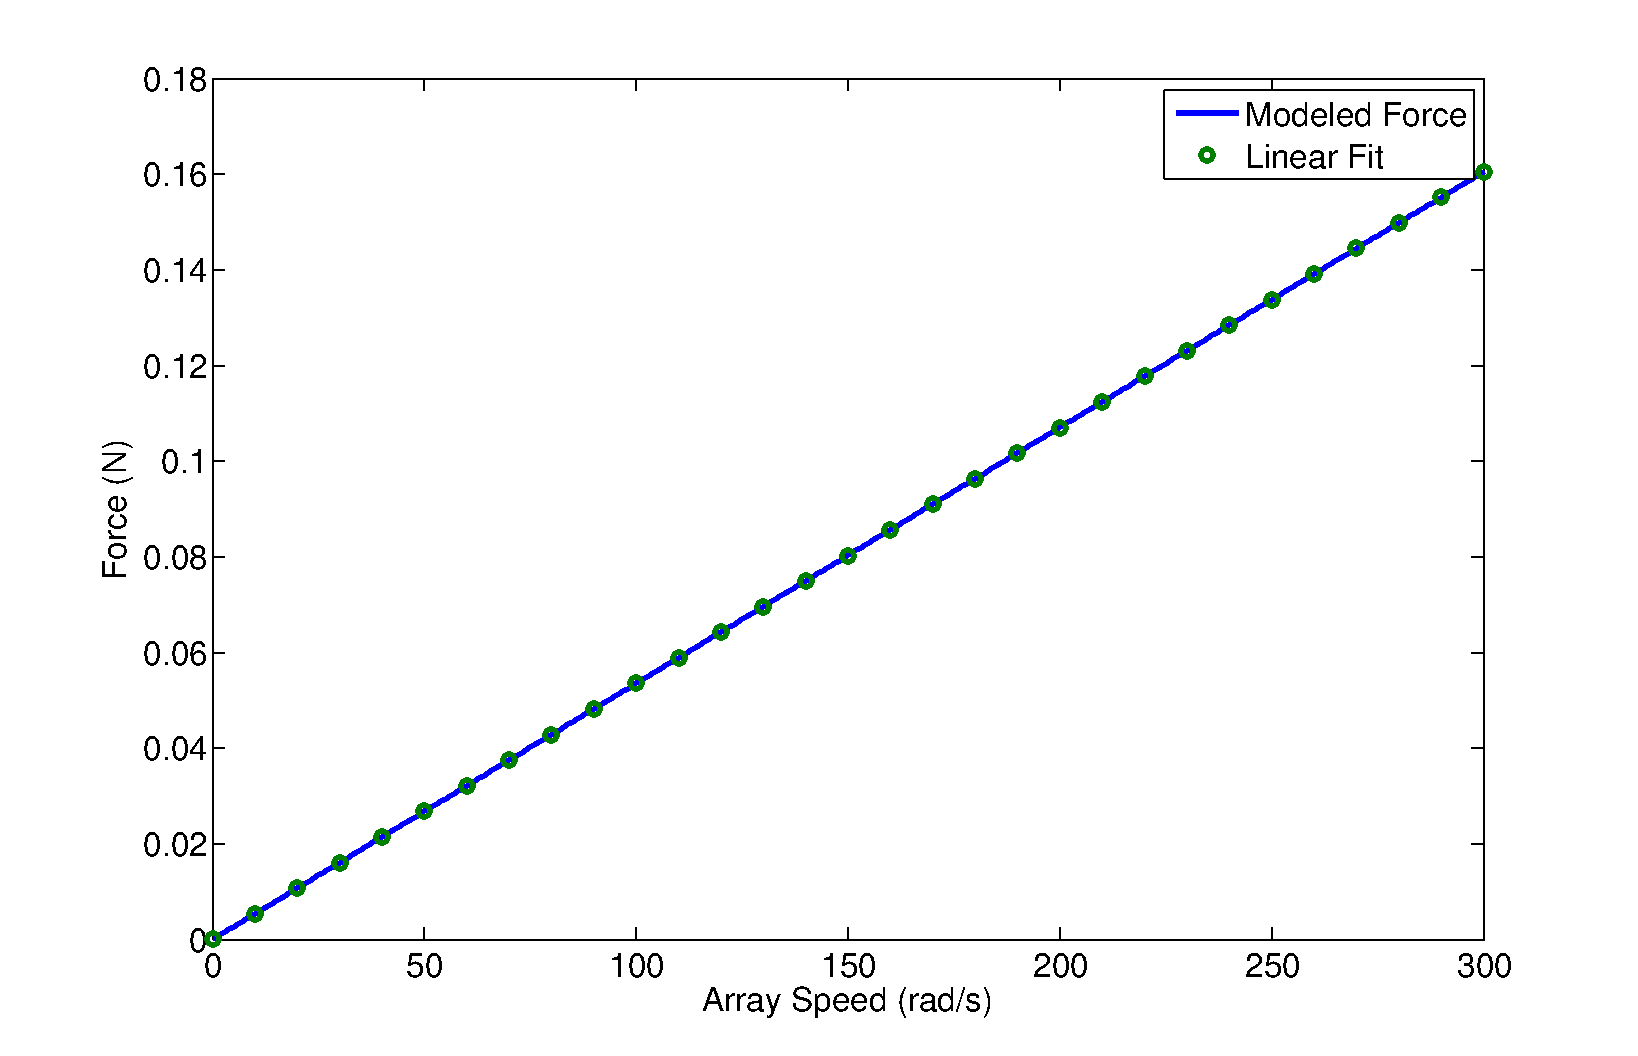
\includegraphics[width = 6cm]{figures/lin_fit.pdf}
\caption{Linear fit between shear force and a magnet array's angular velocity. For the values listed in table \ref{table:values}, the slope is $c = 5.031 * 10^{-4} \frac{N}{rad/s}$}
\label{fig:lin_fit}
\end{figure}


The system kinematics are those of a standard 6 DoF rigid body. 
\begin{equation}\label{eq:rotMrxPropigation}
\dot{R} = \omega^{\times}R
\end{equation}
\begin{equation}\label{eq:RigidBodyKinematics}
\begin{pmatrix} 
I\dot{\omega} \\
m\ddot{x}
 \end{pmatrix}
=
\begin{pmatrix} 
-\omega^{ \times} \left( I\omega \right) \\
0
\end{pmatrix}
+
\begin{bmatrix}
1 & 0 \\
0 & R
\end{bmatrix}
Ju
\end{equation}
where R is the direction-cosine matrix that relates the target coordinate system and the chaser coordinate system. Here, $\omega$ and $x$ are the chaser's angular velocity and position. Note that the chaser angular velocity ($\omega$) is separate from the input speed of coupler i ($\omega_i$.)  $I$ is the chaser's inertia tensor and $m$ is its mass.
\begin{equation}
\label{eq:u_definition}
u = 
\begin{bmatrix}
\omega_1\\
\omega_2\\
...\\
\omega_N
\end{bmatrix}
\end{equation}
The control input $u$ is a column matrix of N speed commands - one for each coupler.

\begin{equation}\label{eq:Jacobian}
J = C\begin{bmatrix} 
d_1^{\times}\left[ \left(1-\beta_1 \right )\hat{a}_1^{\times}\hat{n} + \beta_1\hat{n}\right ]&
d_2^{\times}\left[\left(1-\beta_2 \right )\hat{a}_2^{\times}\hat{n} + \beta_2\hat{n}\right ] &
 ... &
d_N^{\times} \left[\left(1-\beta_N \right )\hat{a}_N^{\times}\hat{n} + \beta_N\hat{n}\right ]
\\

\left(1-\beta_1 \right )\hat{a}_1^{\times}\hat{n} + \beta_1\hat{n}&
\left(1-\beta_2 \right )\hat{a}_2^{\times}\hat{n} + \beta_2\hat{n} &
 ... &
 \left(1-\beta_N \right )\hat{a}_N^{\times}\hat{n} + \beta_N\hat{n}
\end{bmatrix}
\end{equation}
The Jacobian \ref{eq:Jacobian}  imposes constraints on the design of the induction coupler and the chaser's mission.

\begin{itemize}
\item  $\boldsymbol{d}_i{\times}\hat{\boldsymbol{a}}_i$ must be nonzero for at least one array, corresponding to the requirement that all of the spin axes cannot be perpendicular to their moment arms, nor can all $\boldsymbol{d}_i$ be zero (i.e. some of the arrays cannot be at the unlikely location of the target spacecraft's center of mass).
\item  Not all of the spin axes $\hat{\boldsymbol{a}}_i$ can be parallel. If they were, the Jacobian would not be full rank.
\end{itemize}

An induction coupler of this type on a 4 kg spherical spacecraft of radius 0.1 m, can generate a linear acceleration of
$a = 2*10^{-3} \frac{m}{s^2}$ 
and an angular acceleration of 
$\alpha = 9*10^{-3} \frac{rad}{s^2}$. 
These values, while modest, allow an inspection vehicle to overcome typical LEO perturbation forces
\cite{wertz2011space}
 and move slowly over the surface of the ISS to inspect it. These values are based on the small prototype comprised of COTS components and an induction coupler as described above, with only three magnet arrays. Using additional arrays and using more efficient hardware like high-speed brushless motors are two straightforward ways to increase the capabilities in this example.

A three-array inspection spacecraft performing a maneuver near a flat surface illustrates the capabilities of the induction-coupler system. 

The present analysis assumes that the inspection spacecraft maintains a small constant distance from the surface. The analysis assumes that the force normal to the surface can be ignored, so all motion remains in the plane parallel to the surface. 

The results from a simulation of an inspection vehicle in figures \ref{fig:trajectory} and \ref{fig:theta_and_speeds} with the parameters in table \ref{table:values} demonstrates that a small spacecraft can use induction couplers and an LQR controller to inspect a large area in a 
reasonable amount of time. In the simulation, the inspector traversed path defined by several waypoints that was 3.4 m long and included 90 degrees of heading change. Extending these results, an inspector with a 0.1 m inspection swath could cover the 39 $m^2$ surface of the Destiny ISS module in just under two hours.   

\begin{figure}

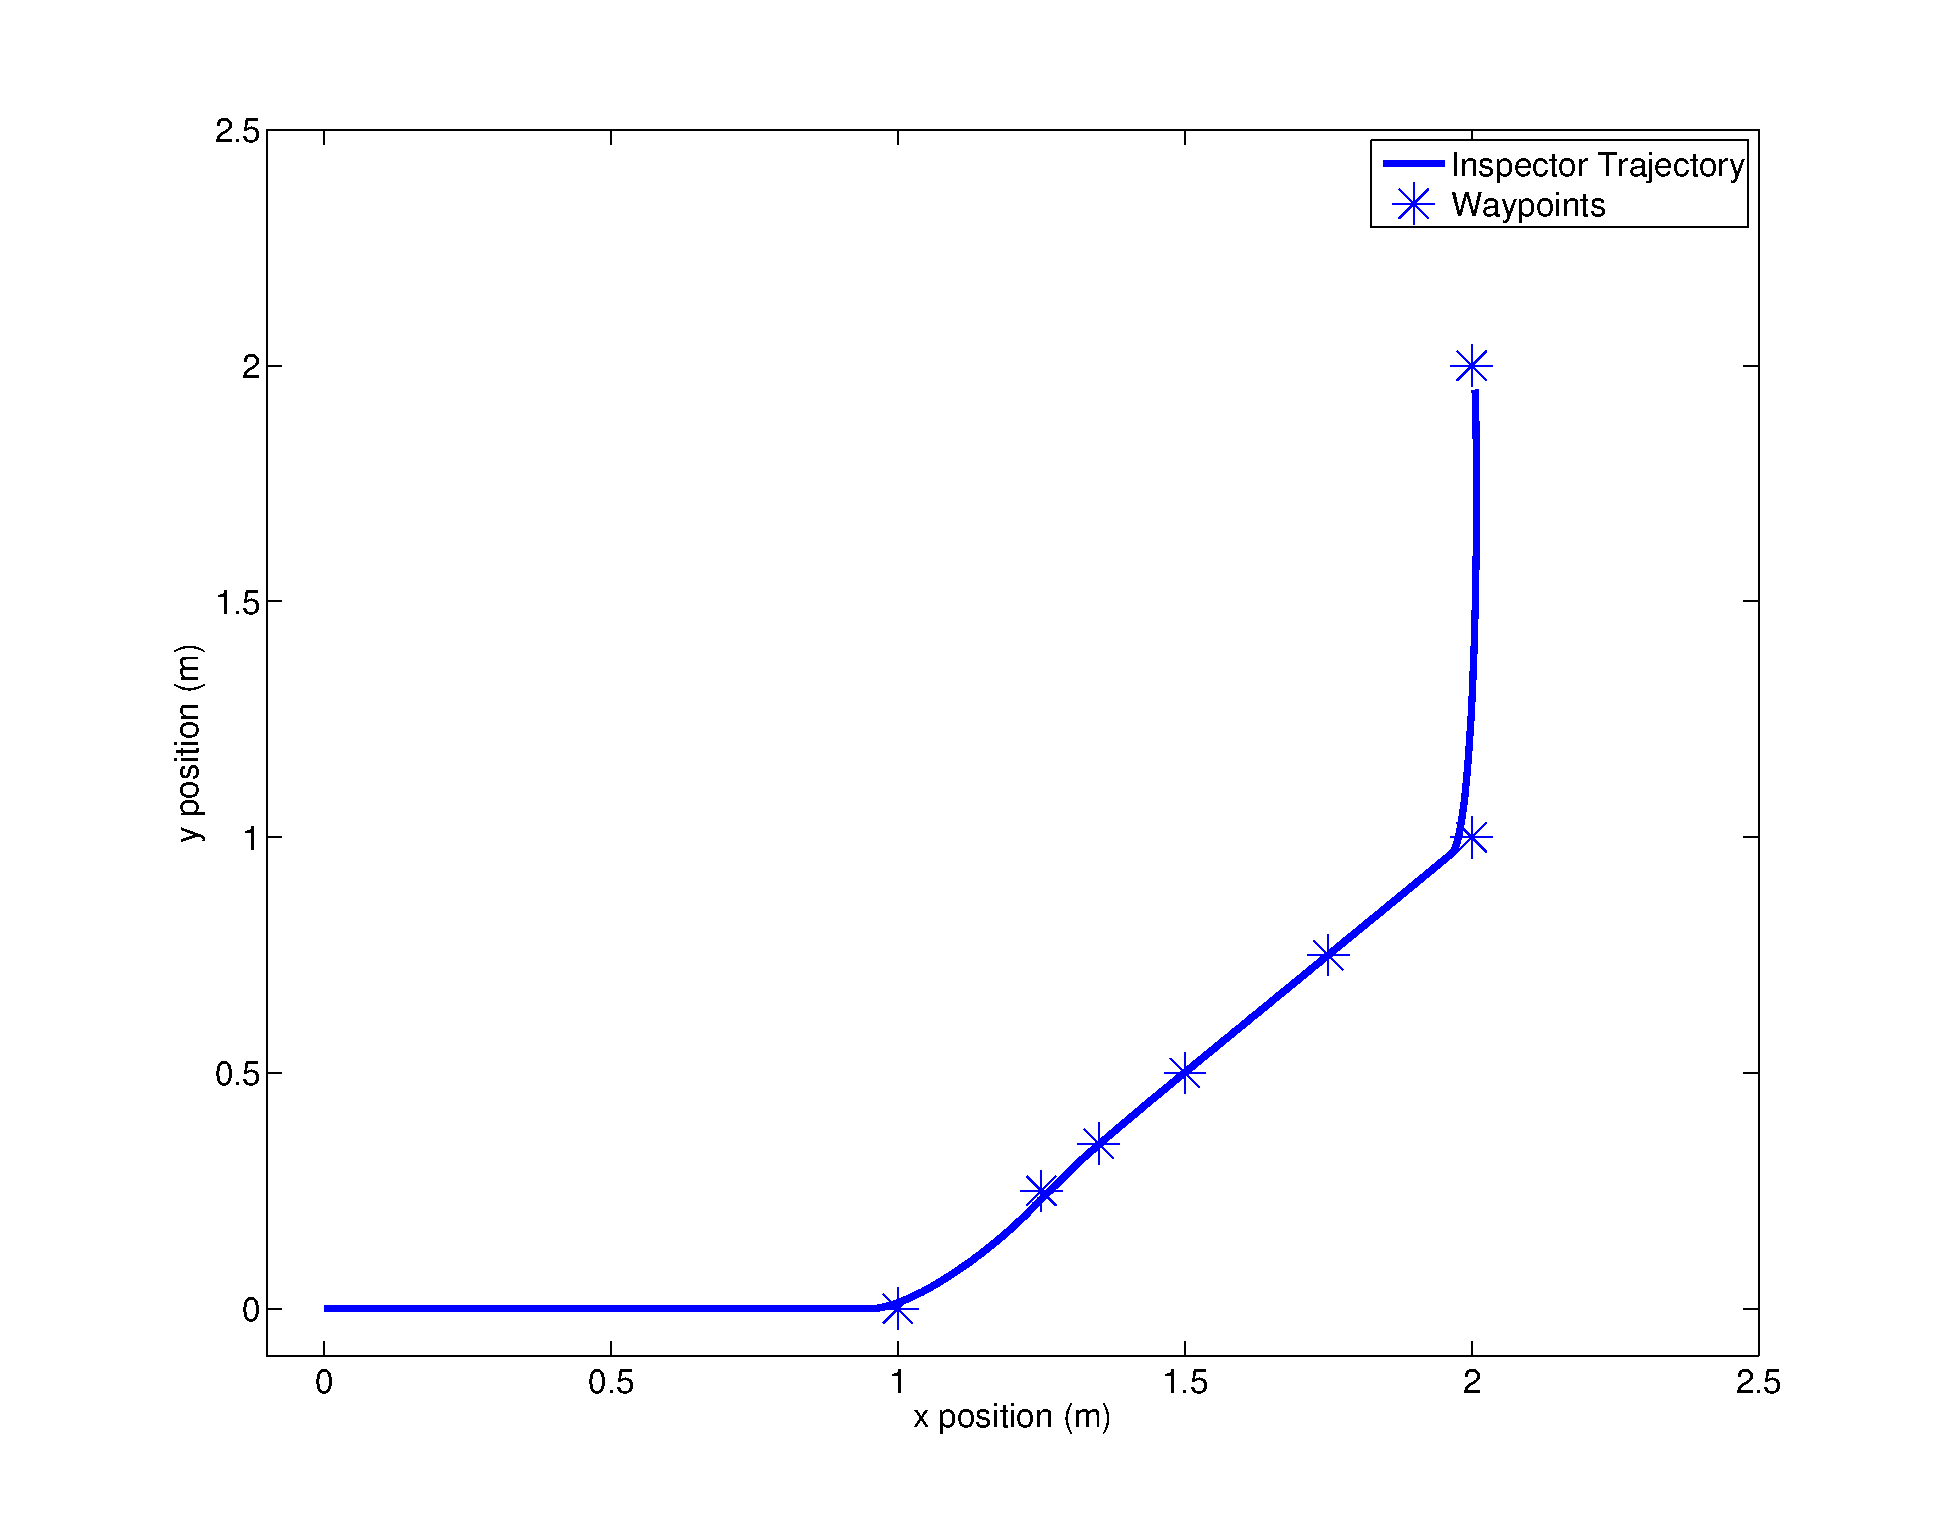
\includegraphics[width = 6cm, height = 6cm ]{figures/sim_trajectory.eps}
\caption{Trajectory of a simulated inspection vehicle. Using conservative parameters A series of waypoints specify a path 3.4 m long with a 90 degree turn. }
\label{fig:trajectory}
\end{figure}

\begin{figure}

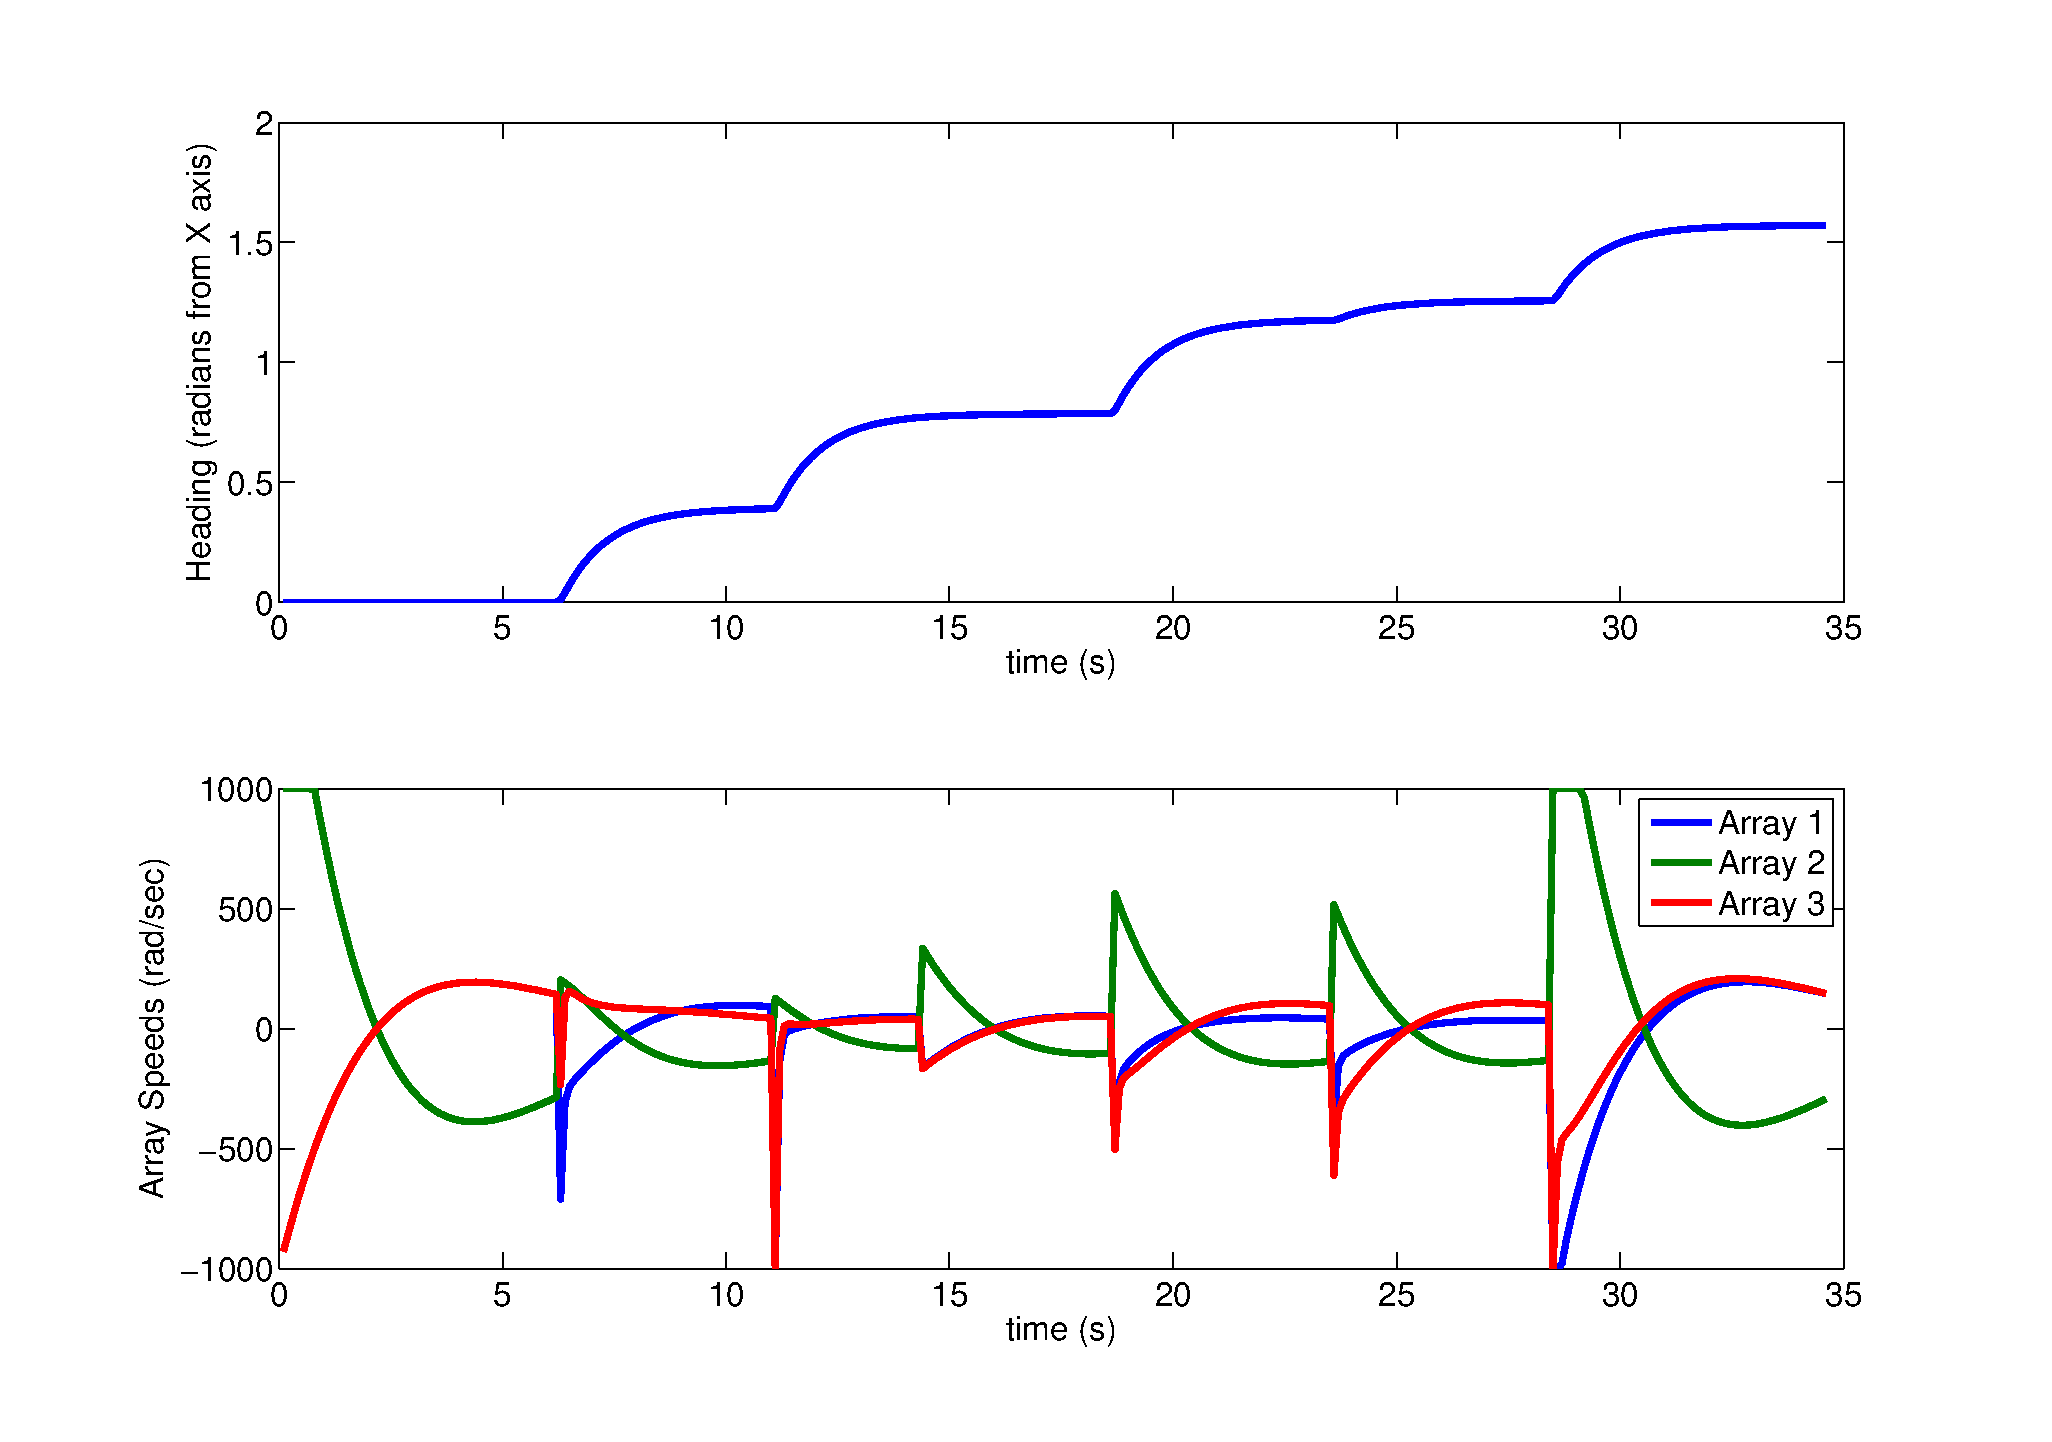
\includegraphics[width = 6cm, height = 6cm ]{figures/heading_and_control_sim.eps}
\caption{Heading and speed for a simulated inspection vehicle. }
\label{fig:theta_and_speeds}
\end{figure}



\begin{table}[ht]
\caption{Model Values} % title of Table
\centering % used for centering table
\begin{tabular}{c c c} % centered columns (4 columns)
\hline\hline %inserts double horizontal lines
Variable & Value & Units\\ [0.5ex] % inserts table 
\hline
%heading

$r_i$ & 0.0127 & m\\  
$r_o$ & 0.0191 & m \\
$B_r$ & 1.42 & T \\
$\mu$ & 1.08 & \\
g & 0.01 & m\\

$\sigma$ & $3.53 * 10^5$ & $\frac{S}{m}$ \\
b & 0.01 & m\\
$m$ & 4 & kg \\
$I$ & 0.16 & kg$m^2$

 \\ [1ex] % [1ex] adds vertical space
\hline %inserts single line
\end{tabular}
\label{table:values} % is used to refer this table in the text
\end{table}


\begin{figure}
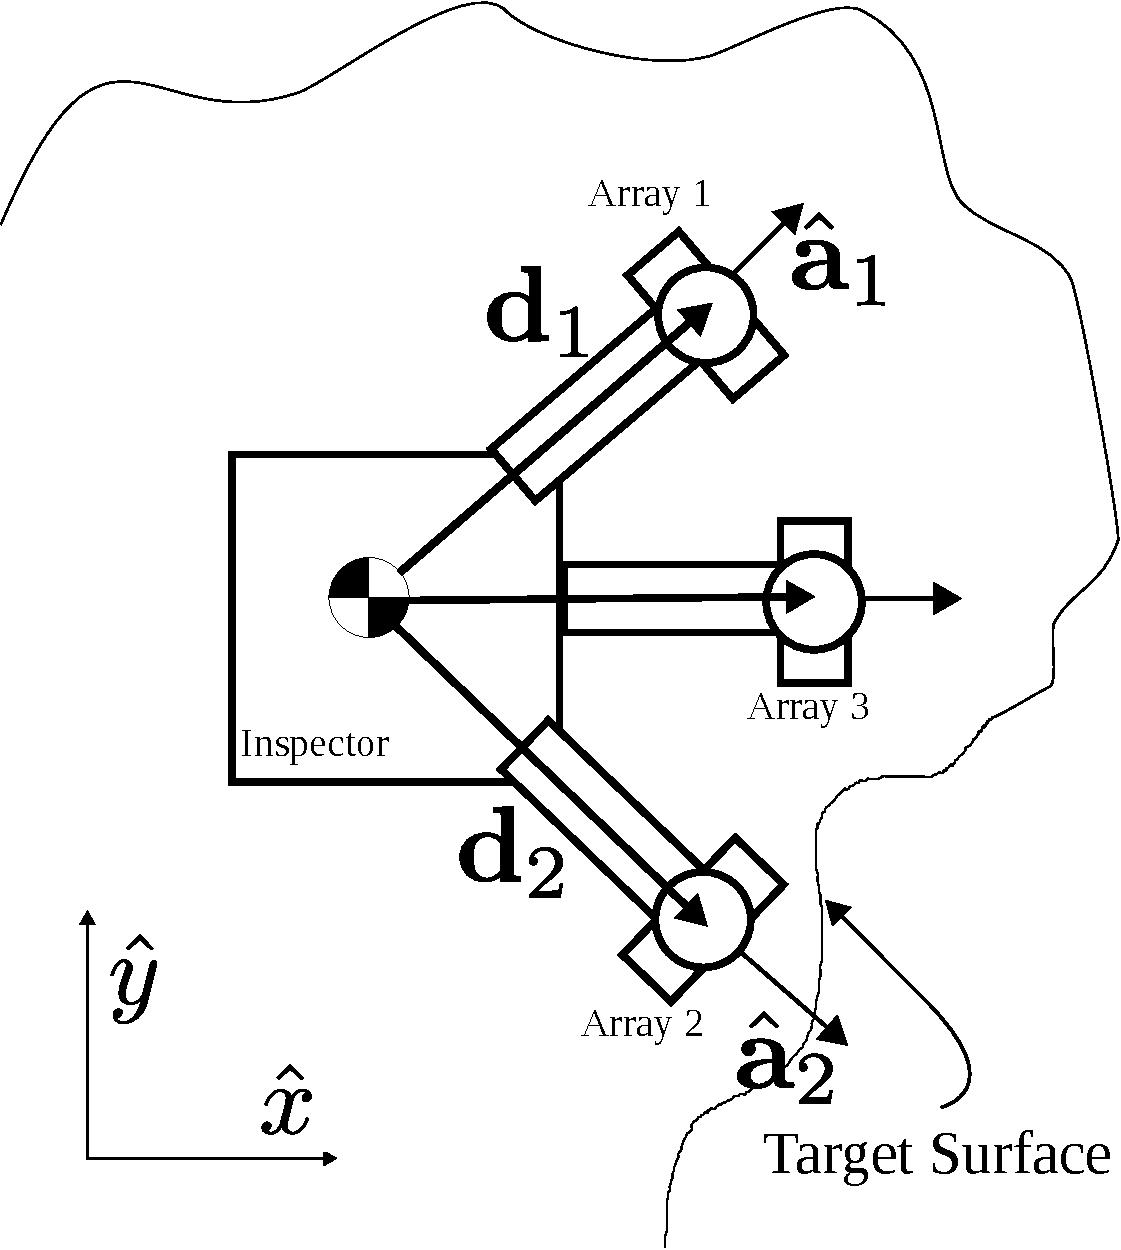
\includegraphics[width = 6cm, height = 6cm ]{figures/surface_locomotion-eps-converted-to.pdf}
\label{fig:sample_coupler}
\caption{Example induction coupler architecture with three single-magnet arrays.}
\end{figure}